\documentclass[11pt,a4paper]{article}

% Packages
\usepackage[utf8]{inputenc}
\usepackage[T1]{fontenc}
\usepackage[margin=2.5cm]{geometry}
\usepackage{graphicx}
\usepackage{xcolor}
\usepackage{tikz}
\usetikzlibrary{shapes.geometric, arrows.meta, positioning, calc, fit, backgrounds}
\usepackage{hyperref}
\usepackage{booktabs}
\usepackage{enumitem}
\usepackage{fancyhdr}
\usepackage{titlesec}
\usepackage{float}
\usepackage{parskip}

% Colors
\definecolor{primary}{RGB}{41, 128, 185}
\definecolor{secondary}{RGB}{52, 73, 94}
\definecolor{accent}{RGB}{231, 76, 60}
\definecolor{success}{RGB}{39, 174, 96}
\definecolor{warning}{RGB}{241, 196, 15}

% TikZ styles
\tikzstyle{component} = [rectangle, rounded corners, minimum width=2.5cm, minimum height=0.8cm, text centered, draw=primary, fill=primary!10, font=\small]
\tikzstyle{server} = [rectangle, rounded corners, minimum width=2cm, minimum height=0.7cm, text centered, draw=success, fill=success!10, font=\small]
\tikzstyle{client} = [rectangle, rounded corners, minimum width=2cm, minimum height=0.7cm, text centered, draw=accent, fill=accent!10, font=\small]
\tikzstyle{monitor} = [rectangle, rounded corners, minimum width=2cm, minimum height=0.7cm, text centered, draw=warning, fill=warning!10, font=\small]
\tikzstyle{arrow} = [thick,->,>=Stealth]

% Header and footer
\pagestyle{fancy}
\fancyhf{}
\fancyhead[L]{EUMaster4HPC Challenge -- Team 8}
\fancyhead[R]{Evaluation Report}
\fancyfoot[C]{\thepage}
\renewcommand{\headrulewidth}{0.4pt}
\renewcommand{\footrulewidth}{0.4pt}

% Hyperref setup
\hypersetup{
    colorlinks=true,
    linkcolor=primary,
    urlcolor=primary,
}

% Title formatting
\titleformat{\section}
{\normalfont\Large\bfseries\color{primary}}{\thesection}{1em}{}
\titleformat{\subsection}
{\normalfont\large\bfseries\color{secondary}}{\thesubsection}{1em}{}

\begin{document}

%  - - Title Page  - -
\begin{titlepage}
    \centering
    \vspace*{3cm}

    {\Huge\bfseries HPC Benchmark Toolkit\\[0.4cm]}
    {\Large\color{secondary} Challenge Evaluation Report\\[1.5cm]}

    {\large
    \begin{tabular}{rl}
        \textbf{Team:} & 8  -  EUMaster4HPC 2025/2026 \\[0.3cm]
        \textbf{Members:} & Alberto Finardi \\
                          & Giovanni La Gioia \\
                          & Laura Paxton \\
                          & Giulia Lionetti \\[0.3cm]
        \textbf{Platform:} & MeluXina HPC Cluster (LuxProvide) \\
        \textbf{Period:} & September 2025 -- January 2026 \\
    \end{tabular}
    }

    \vfill
    {\large February 2026}
\end{titlepage}

% ============================================================================
\section{Introduction and Overview of the Work Delivered}
% ============================================================================

\subsection{Project Context}

As part of the EUMaster4HPC challenge, our team was tasked with developing a tool for benchmarking Large Language Model (LLM) inference on High-Performance Computing infrastructure. The result is the \textbf{HPC Benchmark Toolkit}: a production-ready, open-source framework that automates the deployment, execution, monitoring, and evaluation of LLM inference benchmarks on the MeluXina supercomputer.

\subsection{What We Built}

The toolkit enables users to declaratively define benchmark experiments through YAML \emph{recipes} and execute them on HPC clusters managed by Slurm with Apptainer containers. The system supports two inference backends - \textbf{Ollama} and \textbf{vLLM} (including multi-node distributed mode via Ray) - and is designed to be extensible to additional services.

At a high level, the framework consists of four major subsystems:

\begin{figure}[H]
\centering
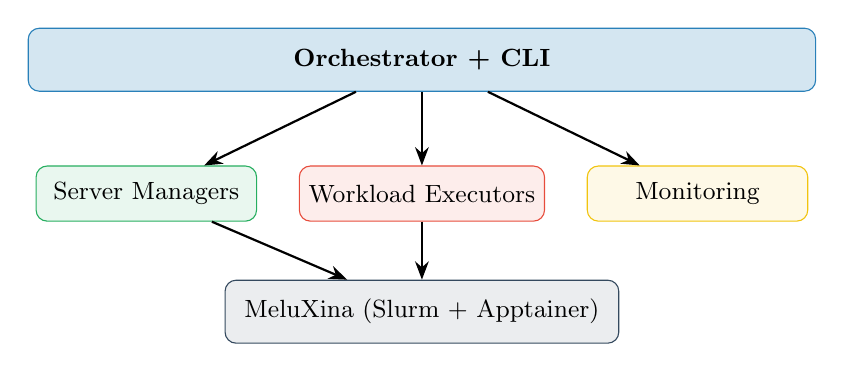
\begin{tikzpicture}[node distance=1.2cm and 2.5cm]
    \node[component, minimum width=10cm, fill=primary!20] (orch) at (0, 2.5) {\textbf{Orchestrator + CLI}};
    \node[server, minimum width=2.8cm] (srv) at (-3.5, 0.8) {Server Managers};
    \node[client, minimum width=2.8cm] (cli) at (0, 0.8) {Workload Executors};
    \node[monitor, minimum width=2.8cm] (mon) at (3.5, 0.8) {Monitoring};
    \node[component, minimum width=5cm, fill=secondary!10, draw=secondary] (hpc) at (0, -0.7) {MeluXina (Slurm + Apptainer)};

    \draw[arrow] (orch) -- (srv);
    \draw[arrow] (orch) -- (cli);
    \draw[arrow] (orch) -- (mon);
    \draw[arrow] (srv) -- (hpc);
    \draw[arrow] (cli) -- (hpc);
\end{tikzpicture}
\caption{High-level architecture of the HPC Benchmark Toolkit.}
\end{figure}

Key capabilities include:
\begin{itemize}[nosep]
    \item \textbf{Recipe-driven experiments}: YAML configurations ensure full reproducibility, with support for parameter sweeps (Cartesian product over concurrency, batch sizes, prompt lengths).
    \item \textbf{Automated Slurm integration}: The CLI generates and submits SBATCH scripts, handles node allocation, and manages container lifecycles.
    \item \textbf{Real-time observability}: Prometheus metrics export and Grafana dashboards (accessed via SSH tunnels) for live throughput and latency visualization.
    \item \textbf{Distributed benchmarking}: Ray-based tensor parallelism across multiple GPU nodes for large-model vLLM deployments.
    \item \textbf{Comprehensive logging}: Distributed log aggregation from all nodes into structured JSON Lines format.
\end{itemize}

\subsection{How We Evaluate the Results}

We assess the quality of our deliverables along four dimensions:

\begin{enumerate}
    \item \textbf{Functional completeness.} The toolkit successfully runs end-to-end benchmarks on MeluXina for both Ollama and vLLM (single-node and distributed). All seven execution phases - from recipe parsing to report generation - work as designed. Parameter sweeps produce the expected Cartesian product of trials.

    \item \textbf{Metrics quality.} The system collects per-request latencies and computes p50/p90/p99 percentiles, throughput (requests/second), and error rates. Metrics are exported as CSV files for post-hoc analysis. A Prometheus/Grafana stack is also available for live monitoring, though its integration remains basic and would benefit from further refinement.

    \item \textbf{Reproducibility.} Any experiment can be re-run by providing the same recipe YAML file. Recipes are self-contained and capture all parameters needed for a benchmark, preventing configuration drift across runs.

    \item \textbf{Extensibility and code quality.} The codebase follows established design patterns (Factory, Template Method, Strategy). Adding a new inference service requires implementing three classes and registering them - no changes to the core orchestrator. The project includes API documentation, a developer guide, and a comprehensive README.
\end{enumerate}

\textbf{Limitations.} The original project plan included additional deliverables such as an interactive web-based dashboard, advanced load patterns (Poisson arrivals, bursty traffic), and streaming inference benchmarking. These features were descoped during the project because the integration, debugging, and end-to-end testing effort concentrated on a "subset" of the team, leaving insufficient bandwidth to pursue all planned work items - see Table~\ref{tab:workload} and Table~\ref{tab:git-stats} for more details.


% ============================================================================
\section{Work Organisation}
% ============================================================================

\subsection{Timeline and Work Calendar}

The project spanned approximately four months (late September 2025 to late January 2026). Development was organised in four main phases:

\begin{table}[H]
\centering
\begin{tabular}{@{}lp{9.5cm}@{}}
\toprule
\textbf{Period} & \textbf{Activities} \\
\midrule
\textbf{Sep 29 -- Oct 10} \newline \textit{Phase 1: Design} &
Requirements gathering and technical specification. Architecture design, recipe format definition (YAML schema), and initial repository setup. Distribution of responsibilities across modules. \\
\midrule
\textbf{Oct 10 -- Nov 25} \newline \textit{Phase 2: Core dev.} &
Core framework development: orchestrator, server managers, workload executors, and Slurm integration (Alberto). Logging subsystem (Giulia). Initial Prometheus/Grafana setup (Giovanni). Recipe format discussions (Laura). First end-to-end Ollama benchmarks on MeluXina. \\
\midrule
\textbf{Nov 25 -- Dec 28} \newline \textit{Phase 3: Integration} &
Integration of all subsystems into a working end-to-end pipeline. vLLM single-node and distributed (Ray) support. CLI development. Monitoring pipeline rework and dashboard refinement. Extensive testing and debugging on MeluXina. \\
\midrule
\textbf{Jan 2026} \newline \textit{Phase 4: Polish} &
Live metrics pipeline finalisation. Documentation (README, API reference, developer guide, technical report, presentation). Final benchmark executions and validation. \\
\bottomrule
\end{tabular}
\caption{Project timeline and main activities per phase.}
\label{tab:workload}
\end{table}

Table~\ref{tab:git-stats} summarises per-contributor statistics as reported by GitHub (\texttt{Insights $\rightarrow$ Contributors}, ordered by additions).

\begin{table}[H]
\centering
\begin{tabular}{@{}l r r r@{}}
\toprule
\textbf{Contributor} & \textbf{Commits} & \textbf{Additions (++)}  & \textbf{Deletions (--)} \\
\midrule
Alberto Finardi  & 13 & 19\,722 & 3\,841 \\
Giovanni La Gioia & 26 & 4\,177  & 7\,727 \\
Giulia Lionetti  & 27 & 3\,609  & 1\,238 \\
Laura Paxton     & 17 & 2\,096  & 878   \\
\midrule
\textbf{Total}   & \textbf{83} & \textbf{29\,604} & \textbf{13\,684} \\
\bottomrule
\end{tabular}
\caption{Git contribution statistics (source: GitHub Insights/Contributors).}
\label{tab:git-stats}
\end{table}

\subsection{Distribution of Tasks}

Alberto designed the system architecture and implemented the orchestrator, all server managers (Ollama, vLLM, Ray cluster), all workload controllers and executors, the benchmarking logic, the CLI with interactive recipe creation, the Slurm sbatch generator, the distributed vLLM/Ray support, the monitoring metrics pipeline, and the project documentation (README, API reference, developer guide, technical report, presentation). He also served as integrator, coordinating module interfaces and performing end-to-end testing on MeluXina throughout the project.

Giulia designed and implemented the logging subsystem: the \texttt{BaseLogCollector} abstract interface, the \texttt{TailerLogCollector} with thread-based file tailing, multi-node log aggregation into structured JSON Lines, and the associated validation scripts.

Giovanni configured the initial Docker-based Prometheus and Grafana containers and created dashboard templates for Ollama and vLLM metrics.

Laura contributed to the initial requirements discussion and recipe format definition, and ran a few benchmark executions on MeluXina towards the end of the project.

\begin{table}[H]
\centering
\begin{tabular}{@{}l l p{6.5cm}@{}}
\toprule
\textbf{Member} & \textbf{Primary Role} & \textbf{Key Deliverables} \\
\midrule
Alberto Finardi & Architect, Lead Dev. \& Integrator & System architecture, orchestrator, server managers, workload controllers \& executors, benchmarking logic, CLI, Slurm integration, distributed vLLM/Ray support, monitoring pipeline, documentation, overall integration \\
Giulia Lionetti & Logging & Logging architecture, \texttt{BaseLogCollector} interface, \texttt{TailerLogCollector} implementation, log aggregation, validation scripts \\
Giovanni La Gioia & Monitoring (initial) & Initial Prometheus/Grafana Docker setup and dashboard templates \\
Laura Paxton & Design \& Testing & Participation in requirements, recipe format definition, benchmark runs \\
\bottomrule
\end{tabular}
\caption{Task distribution across team members.}
\end{table}

\subsection{Collaboration Tools and Workflow}

We used GitHub (\texttt{EUMASTERHPC2526-TEAM-8}) with feature branches and pull requests. All members had MeluXina accounts under the same project allocation (\texttt{p200981}). Communication happened through online meetings and asynchronous messaging. Each module exposed a well-defined Python interface (abstract base classes), enabling parallel development with minimal merge conflicts; integration was performed incrementally.

% ============================================================================
\section{What We Gained from the Challenge}
% ============================================================================

\subsection{Technical Skills}

Working on this project provided hands-on experience with a full HPC software stack beyond what is covered in coursework:

\begin{itemize}[nosep]
    \item \textbf{HPC operations}: Slurm scheduling, Apptainer containers, multi-node allocation, and the constraints of shared supercomputer environments (queue times, limited GPU hours, no root access).
    \item \textbf{Distributed systems}: Ray-based distributed vLLM deployment, cluster coordination, cross-node network management, and debugging distributed failures.
    \item \textbf{Observability}: Building a metrics pipeline from in-process counters through Pushgateway, SSH tunnels, and Grafana dashboards.
    \item \textbf{Software architecture}: Designing a modular framework with Factory, Template Method, and Strategy patterns, and maintaining clean interfaces across independently developed subsystems.
    \item \textbf{LLM inference}: Performance characteristics of Ollama vs.\ vLLM, tensor parallelism impact, and the gap between theoretical and real-world GPU throughput.
\end{itemize}

\subsection{Reflections}

The most valuable outcome is the confidence from having built a non-trivial system end-to-end on real HPC infrastructure. Bridging the gap between tutorial examples and a multi-node benchmarking framework on a production supercomputer required solving many unglamorous but important problems: debugging SSH tunnels, handling container bind mounts, managing Slurm job lifecycles, and ensuring metrics flow from cluster nodes to local dashboards. If we were to start over, we would establish more frequent milestone check-ins and allocate more time for comparative benchmarks. The framework we delivered is functional, extensible, and documented - a solid foundation for future work.

% ============================================================================

\end{document}
